\documentclass[compress,hyperref={linkcolor=blue,pdftex,unicode}]{beamer}
\usepackage[utf8]{inputenc}
\usepackage[english,russian]{babel}

\ifpdf
        \usepackage{cmap} % чтобы работал поиск по PDF
\fi

\usepackage{indentfirst}
\usepackage{eurosym}
\usepackage{xspace}
\usetheme{Copenhagen}
\usecolortheme{wolverine}
\useinnertheme{rectangles}
\setbeamerfont{title}{shape=\itshape,family=\rmfamily}
\setbeamercolor{alerted text}{fg=blue}
\setbeamercovered{highly dynamic}
\setbeamertemplate{navigation symbols}{}
\setbeamertemplate{footline}
{%
\rightline{\begin{beamerboxesrounded}[width=.3cm,center]{}\insertframenumber\end{beamerboxesrounded}\vspace*{3pt}}
}

\newcommand{\myhref}[2]{\textcolor{blue}{\href{#1}{#2}}}
\newcommand{\mycompet}[1]{\resizebox{!}{1.76cm}{\includegraphics{#1}}}

\date{29 декабря 2011\,г.}
\author[]{\myhref{mailto:info@electorus.org}{\tt info@electorus.org}}
\title[\tiny Electorus]{Открытая система общественного контроля голосования <<Electorus>>}
\institute[\tiny Интернет-избирком]{Презентация проекта общественного контроля голосования}

\subject{Electorus - открытая система контроля результатов голосования}
\keywords{Electorus, выборы, система контроля, калькулятор, пересчет, счетчик, общественный, elections, control, check, society, civil}

\begin{document}
\large
\section*{Electorus}
\begin{frame}
\titlepage
\end{frame}

\section*{Постановка проблемы}
\begin{frame}
\frametitle{Процесс голосования в России. Проблемы}

\begin{itemize}
\item Низкий уровень доверия к данным ЦИК со стороны граждан, партий и общественных организаций
\item Существует неудовлетворенный запрос граждан на проверку данных ЦИК общественными объединениями и партиями
\end{itemize}
\vspace*{.5cm}

\begin{tabular}{cccc}
\mycompet{meeting1}&\mycompet{meeting2}&\mycompet{meeting3}&\mycompet{meeting4}\\
\end{tabular}
\medskip

\centerline{\fontsize{1mm}{1mm}\selectfont\copyright \myhref{http://creativecommons.org/licenses/by-sa/2.0/}{Creative Commons} \myhref{http://www.flickr.com/photos/andyindesign/6528311309/sizes/z/in/photostream/}{andyindesign} Фотография митинга.}
\end{frame}

\begin{frame}
\frametitle{Существующие платформы (состояние на 29.12.2011)}
\begin{itemize}
\item \textbf{\myhref{http://www.ruelect.com}{ruelect.com}} Данные вводятся анонимно. Выгрузка данных для пересчета --- CSV файл с данными протоколов, загруженных анонимными пользователями.
Расчетные алгоритмы закрыты\footnote{\textbf{\textit{Закрытость алгоритмов делает невозможным их инспекцию с целью выявления 
ошибок в логике, внесенных преднамеренно или случайно.}}}. Упор делается на подсчете  <<украденных для ЕдРо>> голосов
\item \textbf{\myhref{http://egolos.org.ru/}{egolos.org.ru}} Открытые исходные тексты. Стадия --- согласование ТЗ. Последняя активность - 02.2008
\item \textbf{\myhref{http://www.kartaitogov.ru/}{карта итогов выборов}} Возможна выгрузка данных для пересчета --- CSV файл с данными по всем участкам. Алгоритмы расчета и импорта данных ЦИК закрыты${}^1$. Данные ассоциации <<Голос>>
\end{itemize}
\end{frame}

\begin{frame}
\frametitle{Результаты обзора существующих решений (29.12.2011)}
\alert{Существующие IT-решения общественного контроля не отвечают на вопрос о доверии избирателей и партий к результатам подсчета и являются только средством воздействия на общественное мнение.}
\medskip

Ни одно из них не используется политическими партиями.
\vspace*{.25cm}

\begin{tabular}{ccc}
\mycompet{ruelect}&\mycompet{egolos}&\mycompet{itogi}\\
\end{tabular}
\medskip

\textbf{\textit{Вопрос доверия к системе и данным, которые она выдает, является ключевым для успеха проекта. Возможность
внешней проверки работы системы критична для обеспечения доверия к ней.}}
\end{frame}

\begin{frame}
\frametitle{Цель проекта}
Создание платформы контроля подсчета голосов на выборах любых уровней, позволяющей любой партии, общественной организации, инициативной группе лиц \textbf{независимо друг от друга и ГАС <<Выборы>>:}

\begin{itemize}
\item Проводить параллельный ЦИКу подсчет голосов на основании данных наблюдателей
\item Выявлять несоответствия в данных различных наблюдателей и ЦИК
\end{itemize}
\medskip

\alert{Основные нефункциональные требования:}
\begin{itemize}
\item высокий уровень доверия к системе со стороны граждан и общественных организаций
\item минимальные требования к уровню компьютерной грамотности операторов ввода данных
\end{itemize}
\end{frame}

\section*{Решение}
\begin{frame}
\frametitle{Сообщества Electorus --- пересчет голосов на своей системе, сравнение с данными других сообществ}
\begin{itemize}
\item Любой желающий может создать свое <<сообщество Electorus>>, члены которого (они и только они) имеют доступ к вводу протоколов
\item \alert{Каждое сообщество --- это отдельная инсталляция Electorus. Полный контроль администрации сообщества над системой}
\item Интерфейсы для выгрузки данных в другие сообщества (только чтение) и загрузки данных из сторонних сообществ (по запросу администратора)
\item Возможность сравнения данных сообществ
\end{itemize}
\end{frame}

\begin{frame}
\frametitle{Взаимодействие члена сообщества Electorus (наблюдателя) с системой}
\begin{columns}
\begin{column}{.5\textwidth}
\resizebox{!}{\textheight}{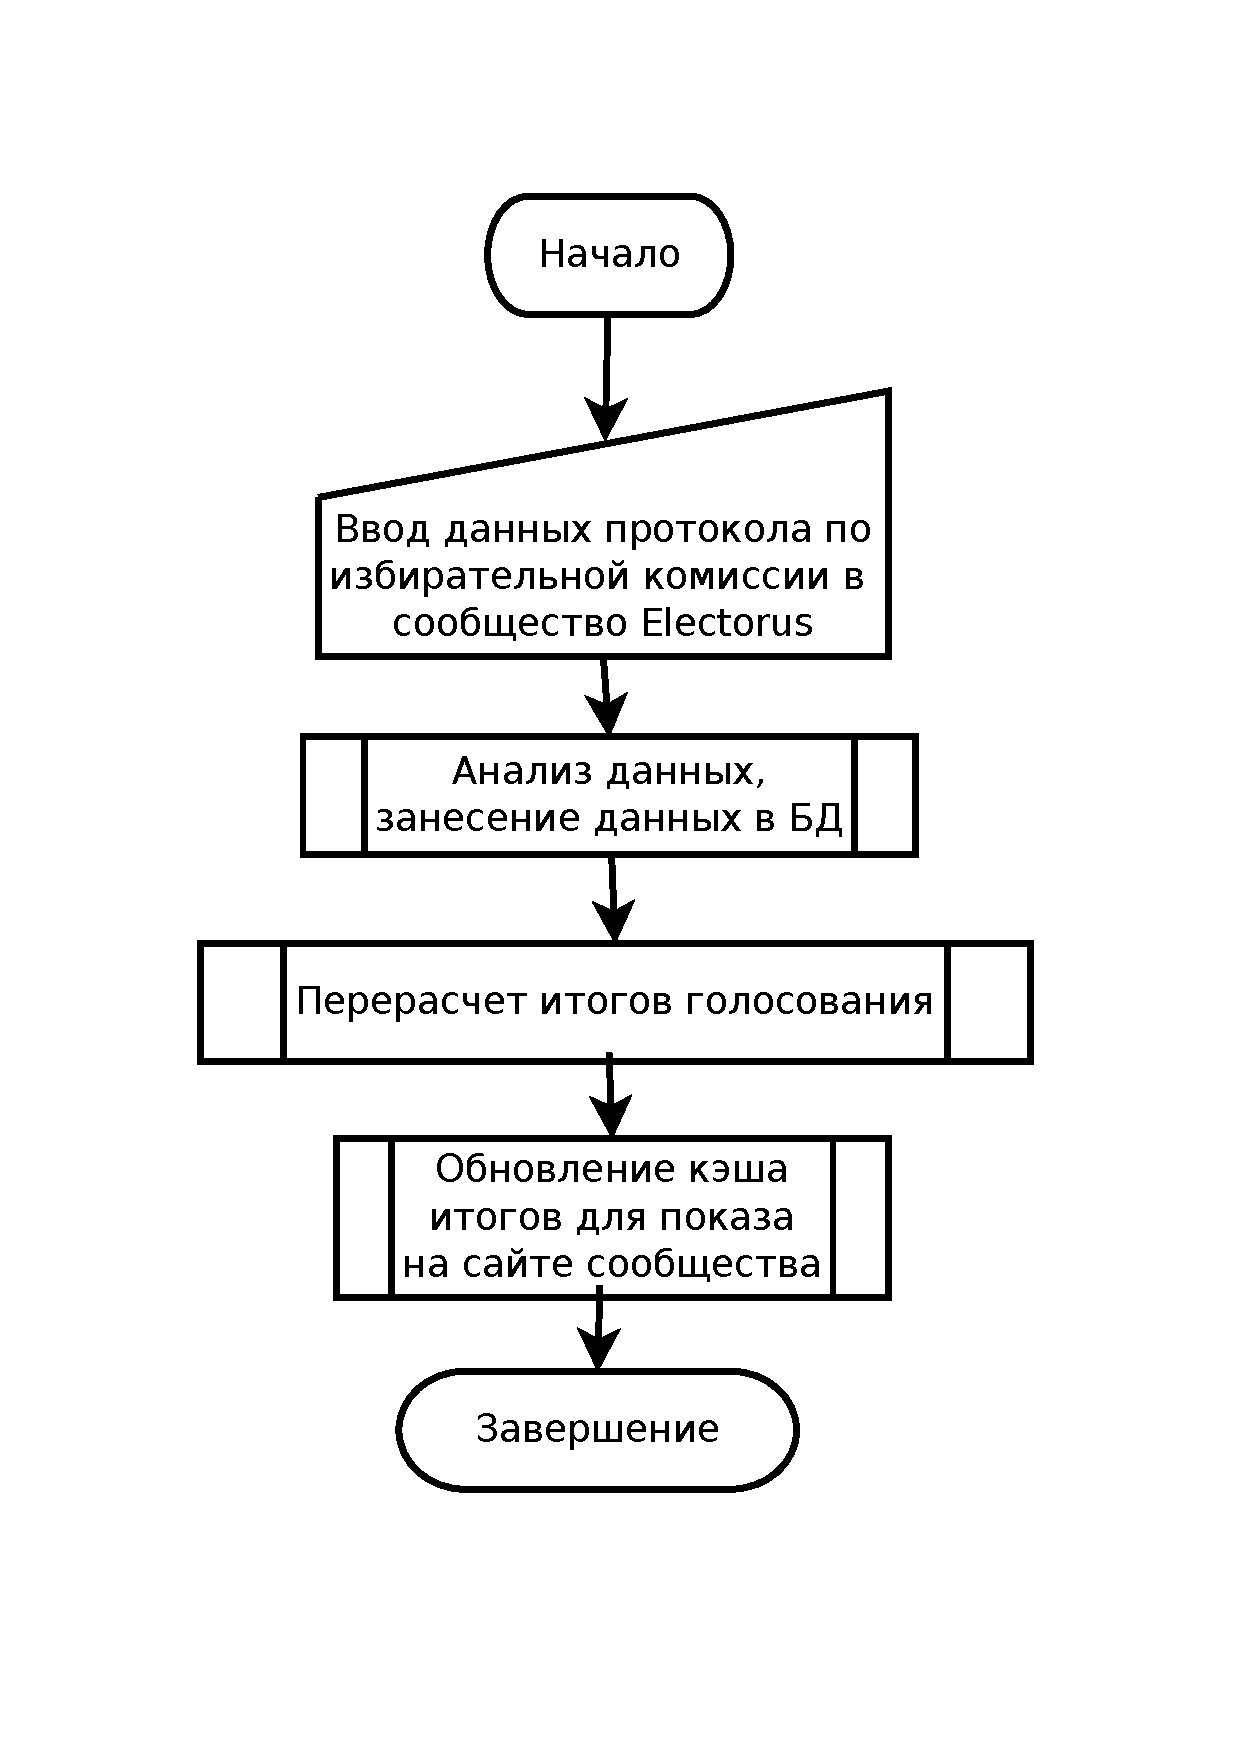
\includegraphics{electro-input}}
\end{column}
\begin{column}{.5\textwidth}
\begin{itemize}
\item Только член сообщества (наблюдатель) может вводить данные. Анонимный ввод не допускается
\item Конечные итоги (результаты выборов по версии сообщества) пересчитываются при поступлении новых данных
\end{itemize}
\end{column}
\end{columns}
\end{frame}

\begin{frame}
\frametitle{Инсталляции сообществ Electorus}
\begin{center}
\resizebox{1.1\textwidth}{!}{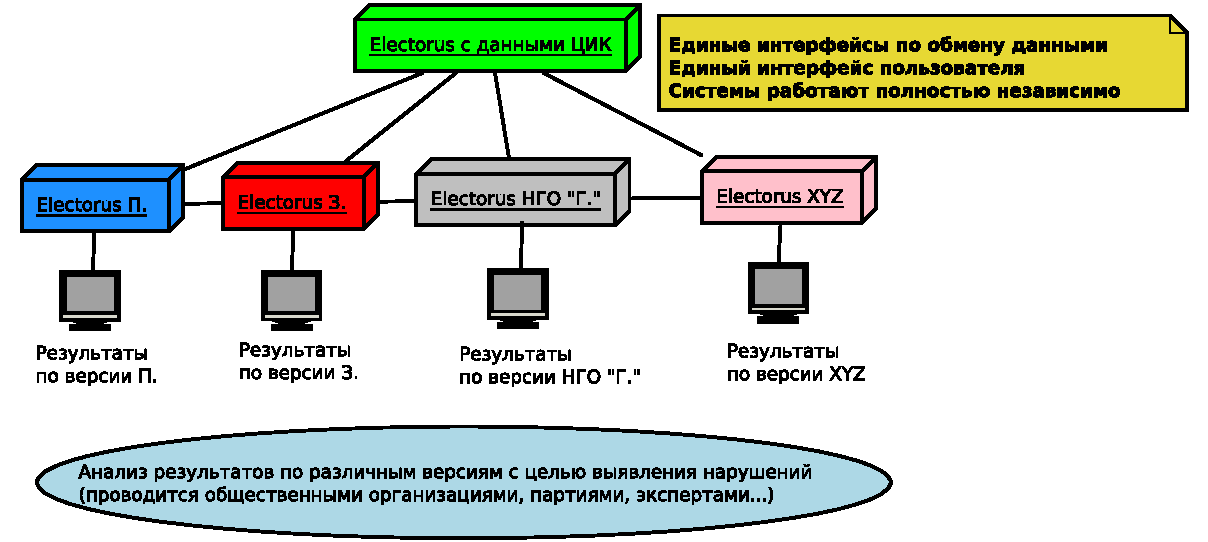
\includegraphics{electorus-ex}}
\end{center}
\end{frame}

\begin{frame}
\frametitle{Довериe к данным системы со стороны граждан и общественных организаций}
\begin{itemize}
\item \alert{Полный контроль сообщества над данными} --- только администрация сообщества контролирует доступ к данным своего сообщества
\item \alert{Выгрузка данных} позволяет проверить расчеты на своей копии системы Electorus и провести \alert{сравнение данных сообществ,} позволяющее выявлять модификации алгоритмов Electorus, внесенные недобросовестными администраторами сообществ
\item \alert{Полностью открытые исходные тексты} делают возможным инспекцию всех алгоритмов системы
\item \alert{Открытая модель разработки} --- к участию в проекте приглашаются все желающие вне зависимости от их политических убеждений. Единственный критерий --- профессионализм в области разработки ПО
\end{itemize}
\end{frame}

\begin{frame}
\frametitle{Ввод данных в систему максимально упрощен}
Сотни тысяч наблюдателей на выборах федерального уровня в РФ. Обучить такое количество пользователей
вводу данных в IT-систему до марта 2012\,г. --- крайне трудоемкая и рискованная задача.
\medskip

\alert{\centerline{Наблюдатель не обязан уметь пользоваться ПК!}}

\begin{itemize}
\item Организация решает использовать Electorus и разворачивает свое сообщество
\item Наблюдатель, получив копию протокола, с использованием любых средств связи (телефон, SMS/MMS, факс, ...) передает данные протокола ответственным лицам в штабе организации
\item Ответственные лица  вводят данные в систему. Копия протокола пересылается наблюдателем в штаб и заносится в Electorus позже
\end{itemize}
\end{frame}

\section*{Выводы}
\begin{frame}
\frametitle{Основные результаты проекта}
\begin{itemize}
\item Каждое сообщество Electorus предлагает свою версию результатов выборов. Граждане
опираются на результаты тех сообществ (партий, общественных организаций), которым они доверяют в большей степени.
\item Возможность использования для выявления нарушений в ходе голосования как в целом по стране, так и на конкретной территории вплоть до УИК, выявления расхождений с социологическими опросами
\item Возможность использования в других государствах
\end{itemize}

\begin{center}
\begin{tabular}{ccc}
\mycompet{stat1}&\mycompet{stat2}&\mycompet{stat3}\\
\end{tabular}
\end{center}
\end{frame}

\begin{frame}
\frametitle{Основные технические риски проекта}
\centerline{%
\begin{tabular}{|p{3.5cm}|p{7cm}|}
\hline
\bf Риск & \bf План снижения риска\\
\hline
Риск не уложиться в крайне сжатые сроки сдачи.&Разбиение задачи разработки на два этапа. Первый --- базовая функциональность, достаточная для ввода данных. Второй --- полнофункциональная версия. Запуск проекта с первой версии.\\
\hline
Обучение персонала & Создание интерфейса ввода данных на самой ранней стадии проекта. Обучение пользователей на макете.\\
\hline
Защита от атак типа DDoS& Администрация сообщества (инсталляции Electorus) отвечает за защиту от атак. Уровень риска подвергнуться такой атаке зависит от организации, которая стоит за сообществом.\\
\hline
\end{tabular}}
\end{frame}

\begin{frame}
\frametitle{Основные вехи проекта}
\small
\centerline{%
\begin{tabular}{|p{1cm}|p{9.5cm}|}
\hline
\bf Даты & \bf Веха (Milestone)\\
\hline
10.01&Старт разработки функционального макета --- ввод данных, права пользователей. 
Старт разработки обучающих материалов. Старт разработки версии 1.0 --- базовой функциональности.\\
\hline
18.01& Готовность функционального макета. Начало тренингов для пользователей--наблюдателей.\\
\hline
26.01& Сдача версии 1.0 в тестовую эксплуатацию. Начало процесса bug fixing'a и разработки версии 1.1. \\
\hline
07.02 & Запуск версии 1.0 в эксплуатацию.\\
\hline
17.02 & Сдача версии 1.1 (конечная версия) в тестовую эксплуатацию. Начало процесса bug fixing'a и уточнения функциональных требований.\\
\hline
24.02 & Сдача версии 1.1 в тестовую эксплуатацию.\\
\hline
02.03 & Запуск версии 1.1 в эксплуатацию.\\
\hline
\end{tabular}}
\medskip

\alert{\centerline{Сроки исполнения: 10.01--02.03}}
\end{frame}

\begin{frame}
\frametitle{Команда разработчиков}
В разработке представленных предложений участвовали ведущие российские специалисты,
имеющие опыт проектирования, создания и развертывания высоконагруженных IT-систем.
\medskip

\textit{\textbf{Готовы приступить к выполнению проекта по запросу политических партий и общественных организаций, намеренных использовать предлагаемую систему на выборах Президента РФ в 2012\,г.}}
\medskip

\centerline{\myhref{mailto:info@electorus.org}{email: \tt info@electorus.org}}
\end{frame}
\end{document}
